\subsection{Secondo Test}

Sfruttando lo stesso script \textit{Python} del primo test, si analizzano le capacità
dell'algoritmo \textit{K2} nel ricondurre i campioni della distribuzione alla distribuzione
originale stessa. Per fare ciò si utilizza la misura di differenza tra le reti bayesiane definita
al punto 1.2, e si analizza la variazione di tale misura al variare del numero di campioni, del
numero massimo di dipendenze condizionali per ogni nodo e dell'euristica utilizzata.

\subsubsection{Risultati}

\begin{figure}[h]
    \centering
    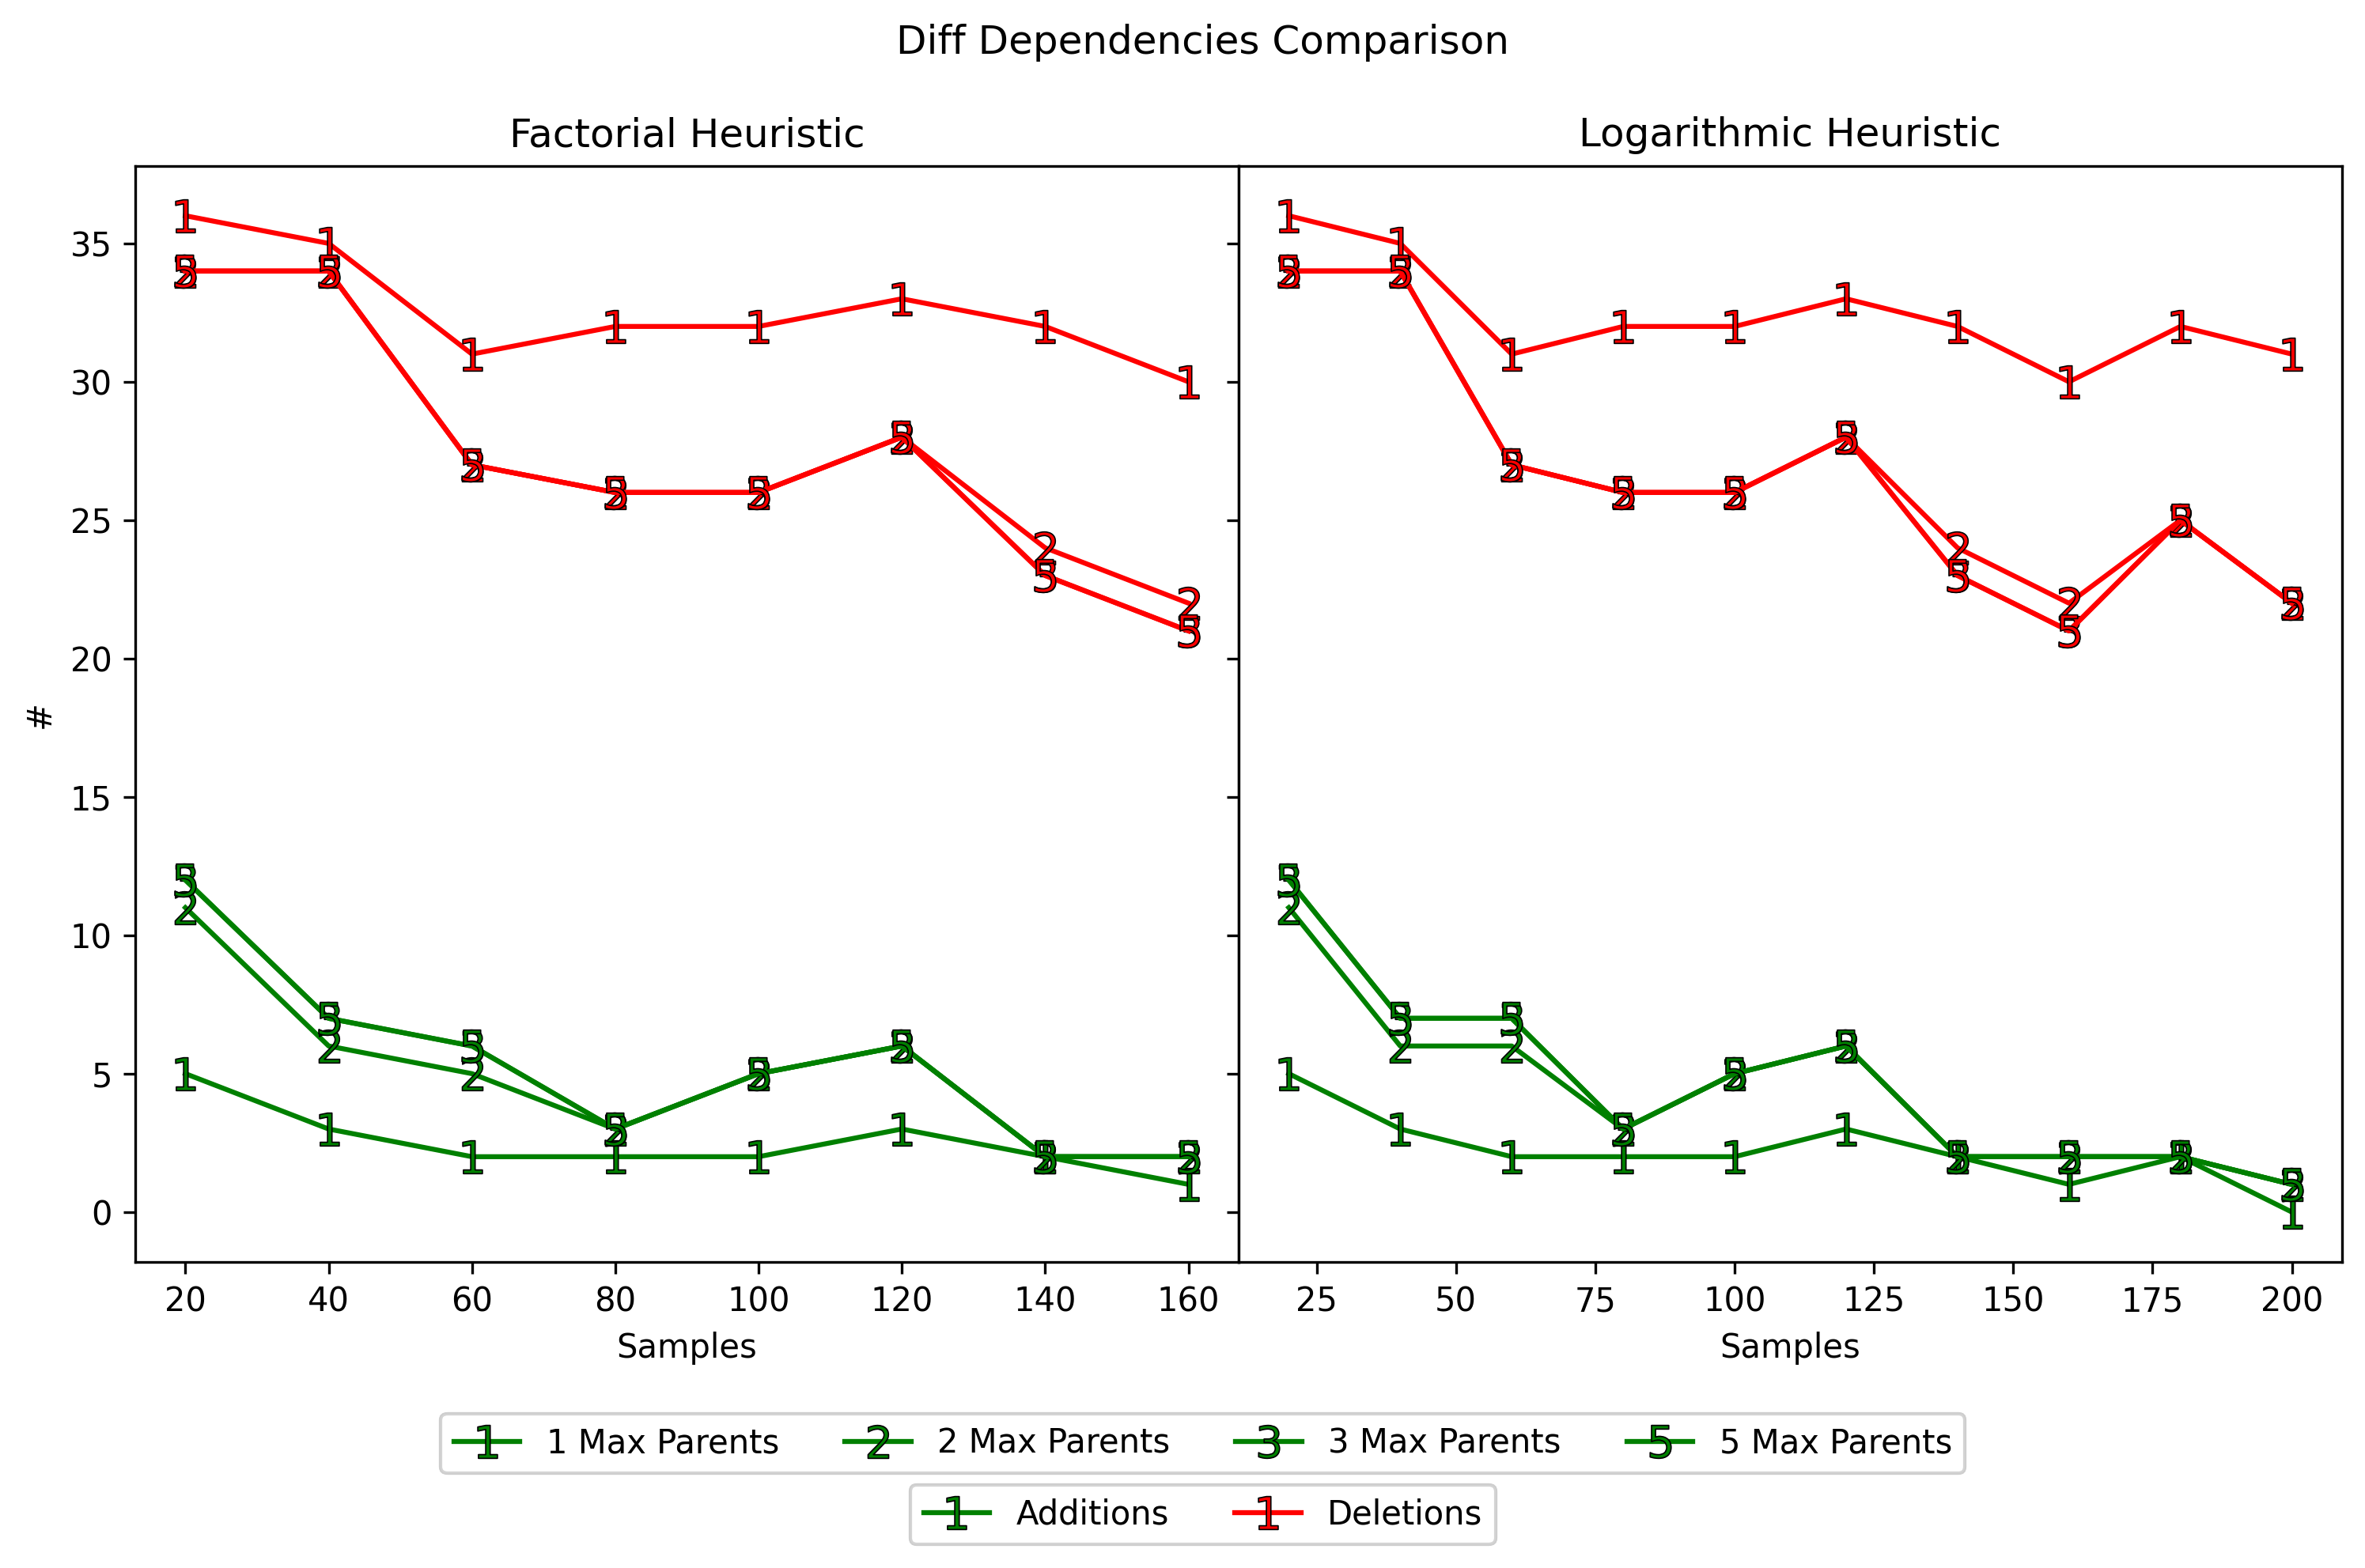
\includegraphics[width=0.9\textwidth]{diffs_deps.png}
    \caption{grafico che rappresenta il numero di dipendenze in eccesso e difetto rispetto alla rete
        originale all'aumentare del numero dei campioni}
    \label{fig:test2}
\end{figure}

I risultati rappresentati in figura \ref{fig:test2} dimostrano che non c'è alcuna differenza
relativamente all'analisi tra l'utilizzo dell'euristica fattoriale e logaritmica, trascurando il
fatto che la variante logaritmica non fallisce dopo 160 campioni. Comunque in entrambi casi
possiamo osservare che aumentando il numero di campioni le discrepanze tra le reti diminuiscono.
Analizzando invece il comportamento al variare del numero massimo di dipendenze si nota che con
tale limite impostato a 1 si ha la possibilità di ottenere reti con meno dipendenze aggiunte, a
discapito di quelle rimosse che risultano maggiori rispetto agli altri limiti; con limiti più alti
(2, 3 e 5) si hanno comportamenti simili che tendono a ridurre il più possibile il numero di
dipendenze in eccesso/difetto. Notiamo comunque che l'algoritmo fatica molto più ad aggiungere
nuove dipendenze rispetto a rimuoverne. In figura \ref{fig:test2:2} si possono osservare le reti
generate.

\begin{figure}
    \centering
    \subfloat[\centering Con 20 campioni]{{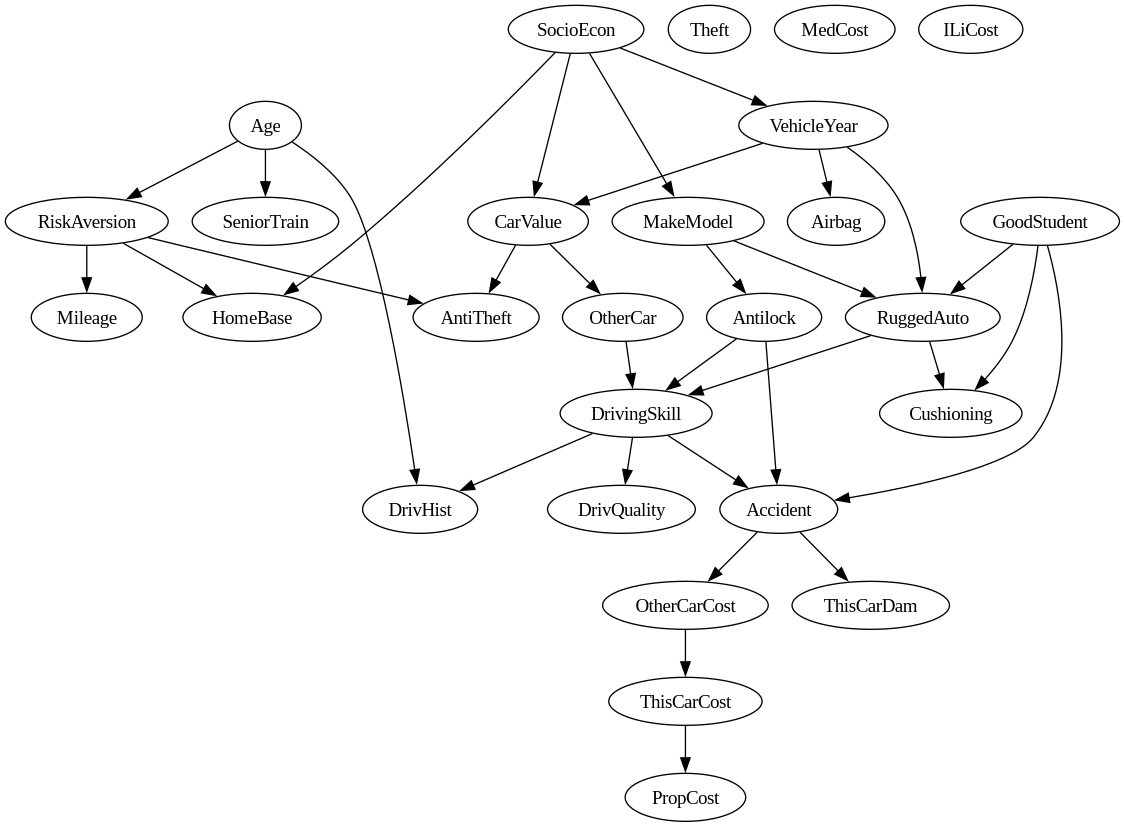
\includegraphics[width=8cm]{graph_20.png} }}
    \qquad
    \subfloat[\centering Con 200 campioni]{{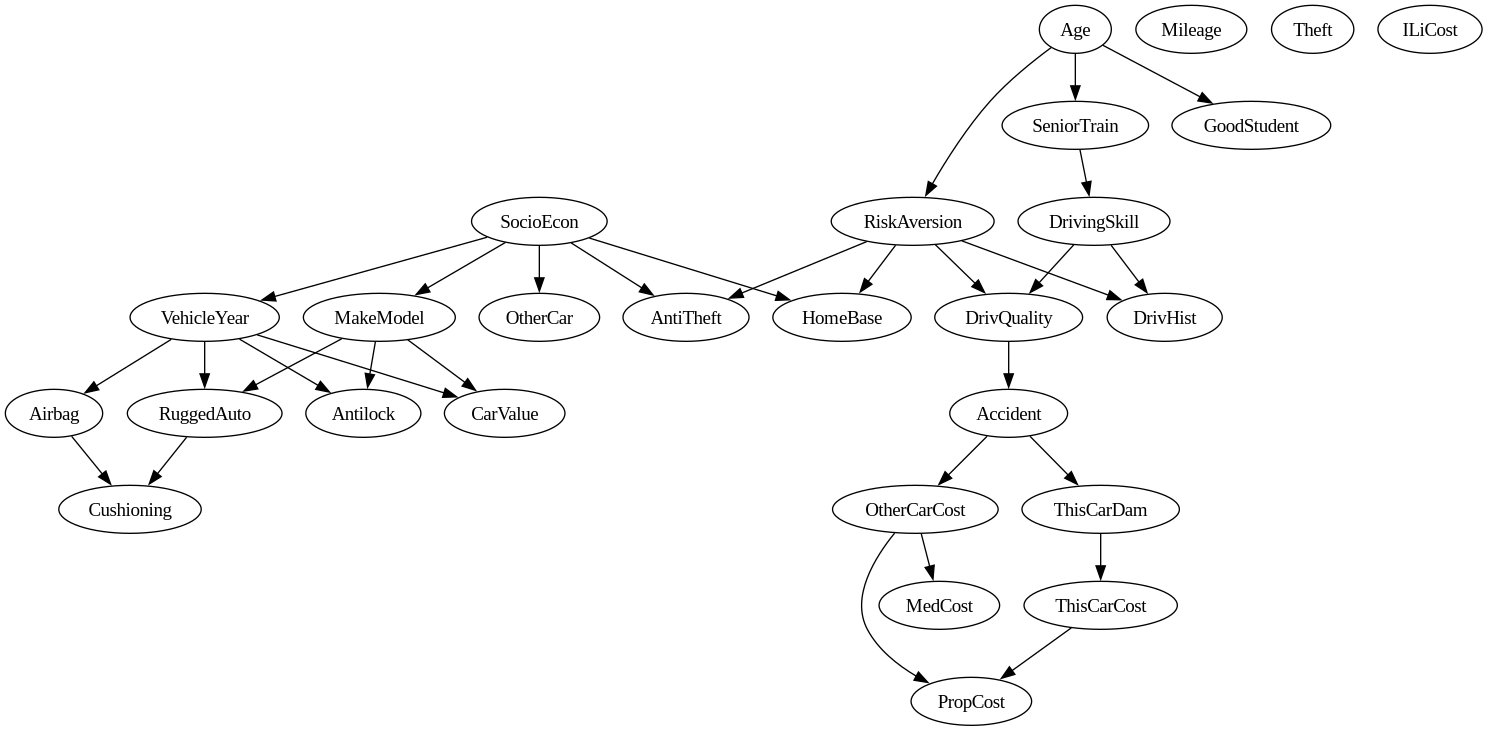
\includegraphics[width=8cm]{graph_200.png} }}
    \caption{Reti bayesiane generate con massimo 5 padri per nodo; è possibile confrontare questi
        grafi con quello originale disponibile all'indirizzo \url{https://www.bnlearn.com/bnrepository/insurance/insurance.svg}}
    \label{fig:test2:2}%
\end{figure}

